%%%%%%%%%%%%%%%%%%%%%%%%%%%%%%%%%%%%%%%%%%%%%%%%%%%%%%%%%%%%%%%%%%%%%%%%
% xfacIntro
%%%%%%%%%%%%%%%%%%%%%%%%%%%%%%%%%%%%%%%%%%%%%%%%%%%%%%%%%%%%%%%%%%%%%%%%

%%% PREAMBLE
\documentclass[10pt]{beamer}
\usetheme{Warsaw}%Berkeley
\usecolortheme{seagull}

%%% General
\usepackage{fixltx2e}

%%% Graphics
\usepackage{graphicx}
\usepackage{wallpaper}
\usepackage[absolute,overlay,verbose]{textpos}

%%% Figures
\usepackage[font=footnotesize]{caption}
\usepackage{subcaption}

\title{MAV Landing Simulation }
\author{Nathan I. Madsen}
\institute{ECEn 674\\Brigham Young University}
\date{Dec 8, 2013}

\begin{document}
{
  \usebackgroundtemplate{%
    \parbox[c][\paperheight][c]{\paperwidth}{%
      %% \begin{textblock*}{20mm}(18mm,47mm)
      %%   \centering\includegraphics[height=1.2in]{img/MERSLogo.png}
      %% \end{textblock*}
      %% \begin{textblock*}{20mm}(83mm,50mm)
      %%   \centering\includegraphics[height=1in]{img/BYULogo.png}
      %% \end{textblock*}
    }
  }
  \frame{\titlepage}
}
\section{Introduction}
\begin{frame}
  \frametitle{Project Goals}
    \begin{itemize}
    \item Model the physics of landing gear
    \item Implement the model in simulation
    \item Create autopilot for landing  
    \end{itemize}
    \begin{figure}[h]
      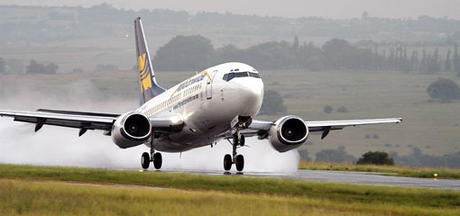
\includegraphics[width=0.75\textwidth]{img/plane-landing.jpg}
      %\caption{Plane Landing}
    \end{figure}

\end{frame}

\begin{frame}
  \frametitle{Model For Landing Gear}
  \begin{columns}[c]

    \column{.5\textwidth}
    \begin{itemize}
    \item 3 wheels, one in front, two in back
    \item Simple spring with damper in body $z$ direction
    \item Compression calculated using position and attitude of aircraft
    \item Friction in horizontal plane split into two components
    \item Force from spring produces torque about and force toward center of mass
    \end{itemize}

    \column{.5\textwidth}
    \begin{figure}[h]
      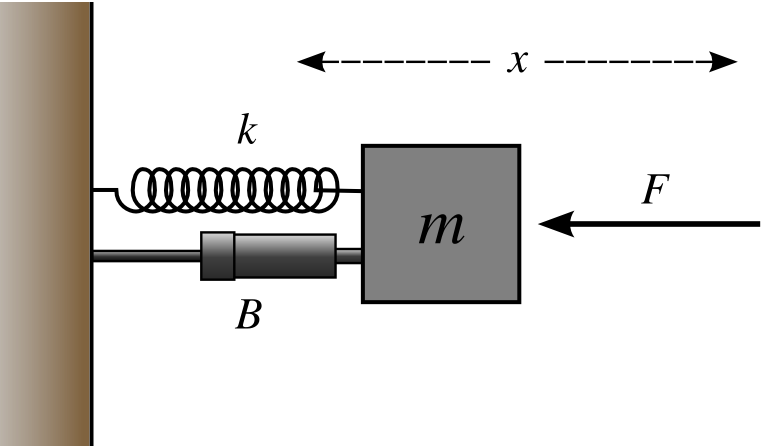
\includegraphics[width=0.75\textwidth]{img/Mass-Spring-Damper.png}
    \end{figure}
    \begin{figure}[h]
      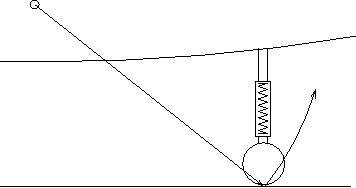
\includegraphics[width=0.75\textwidth]{img/landDiag.png}
    \end{figure}
  \end{columns}
\end{frame}


\begin{frame}
  \large
  \frametitle{Aircraft Control}
  \begin{itemize}
  \item Maintain roll and yaw at zero
  \item At 10 meters altitude, cut throttle and hold 10 degree pitch
  \item After all three wheels on the ground, start applying the brake gradually
  \item Can maintain control in headwind and crosswind (mostly)
  \end{itemize}
\end{frame}

\begin{frame}
  \frametitle{Implementation of Model}
  \begin{itemize}
  \item Added three states to simulation model, offsets for each landing wheel
  \item Added one controllable variable, the brake
  \item Compression calculated using position and attitude of aircraft
  \item Force and torque of spring and damper added to the forces and moments file
  \item Multiple views added to the simulation
  \item Crash conditions added
  \end{itemize}
  
  \begin{figure}[h]
    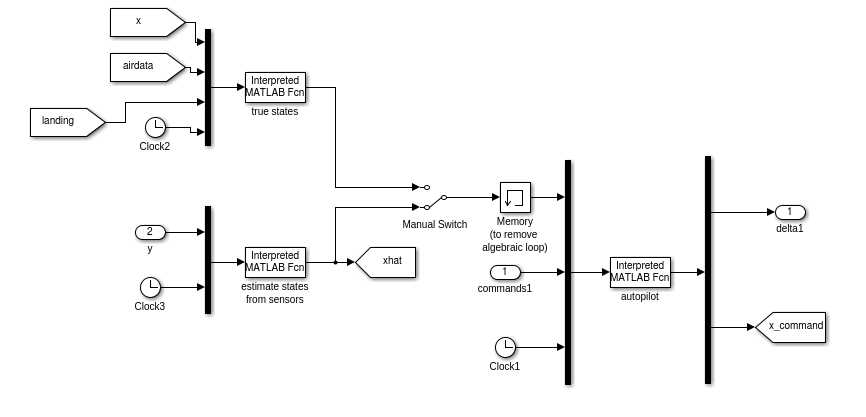
\includegraphics[width=0.75\textwidth]{img/simulinkDiag.png}
  \end{figure}
\end{frame}

\begin{frame}
  \frametitle{Simulation Videos}
\end{frame}

\begin{frame}
  \frametitle{Challenges}
  \begin{columns}[c]
    
    \column{.5\textwidth}
    \begin{itemize}
    \item Suspension
    \item Damping 
    \item Propellor model 
    \item Low-pass filter on difference for damper
    \item Stable in torque and in vertical force
    \item Friction at low velocities
    \end{itemize}
    \column{.5\textwidth}
    \begin{figure}[h]
      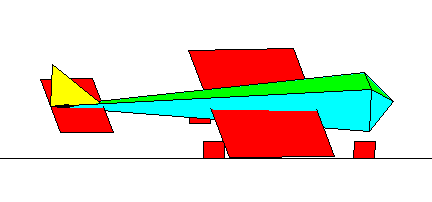
\includegraphics[width=\textwidth]{img/crash1.png}
    \end{figure}
    \begin{figure}[h]
      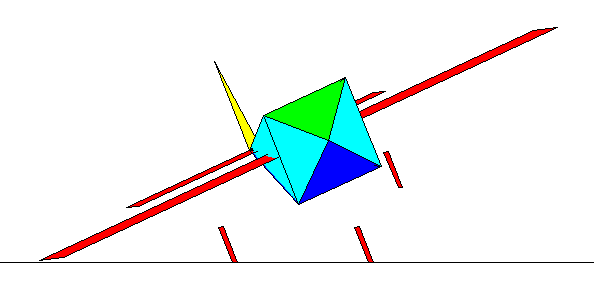
\includegraphics[width=\textwidth]{img/crash2.png}
    \end{figure}
  \end{columns}
\end{frame}



\end{document}
